% Promotional poster for PyCon US 2026
% Breaking the Speed Limit: Fast Statistical Models with Python 3.14, Numba, and JAX

\documentclass[final]{beamer}

\usepackage[T1]{fontenc}
\usepackage{lmodern}
\usepackage[size=custom,width=120,height=72,scale=1.0]{beamerposter}
\usetheme{gemini}
\usecolortheme{imsa}
\usepackage{booktabs}
\usepackage{graphicx}
\usepackage{tikz}
\usetikzlibrary{positioning}
\usepackage{xcolor}

\definecolor{paper}{HTML}{FFF8F2}
\definecolor{ink}{HTML}{17202A}
\definecolor{muted}{HTML}{5F6B74}
\definecolor{cityured}{HTML}{B01117}
\definecolor{cityumaroon}{HTML}{981B49}
\definecolor{cityuorange}{HTML}{E07541}
\definecolor{cityugold}{HTML}{D99A1E}
\definecolor{numba}{HTML}{2F7D32}
\definecolor{jaxberry}{HTML}{B51E59}
\definecolor{threadteal}{HTML}{1F7A8C}

\setbeamercolor{background canvas}{bg=paper}
\setbeamercolor{normal text}{fg=ink}
\setbeamercolor{block title}{fg=cityured,bg=white}
\setbeamercolor{block body}{fg=ink,bg=white}
\setbeamercolor{block alerted title}{fg=cityured,bg=cityuorange!15}
\setbeamercolor{block alerted body}{fg=ink,bg=cityuorange!7}
\setbeamercolor{heading}{fg=cityumaroon}

\newlength{\sepwidth}
\newlength{\colwidth}
\setlength{\sepwidth}{0.014\paperwidth}
\setlength{\colwidth}{0.232\paperwidth}
\newcommand{\separatorcolumn}{\begin{column}{\sepwidth}\end{column}}

\newcommand{\bigstat}[3]{%
  \begin{minipage}[t]{0.31\linewidth}
    {\Huge\bfseries\color{#1} #2}\\[-0.15em]
    {\small\color{muted} #3}
  \end{minipage}
}

\newcommand{\captiontext}[1]{%
  \vspace{-0.5em}
  {\footnotesize\color{muted} #1}
}

% Poster text wrapping: hyphens none; overflow-wrap normal; word-break normal.
\hyphenpenalty=10000
\exhyphenpenalty=10000
\sloppy
\emergencystretch=2em

\title{Breaking the Speed Limit}
\subtitle{Fast statistical models with Python 3.14, Numba, and JAX}
\author{Wenxin Jiang \and Jian Yin}
\institute[shortinst]{Department of Biostatistics, City University of Hong Kong \samelineand PyCon US 2026}

\begin{document}
\begin{frame}[t]
\begin{columns}[t]
\separatorcolumn

\begin{column}{\colwidth}
  \begin{alertblock}{Thesis}
    Simulation is how statisticians write tests when real data has no answer
    key.

    \vspace{0.35em}
    \textbf{Laptop} defines trust. \textbf{Server CPU} tests scale.
    \textbf{A100} matters only after the workload becomes GPU-shaped.
  \end{alertblock}

  \begin{block}{Simulation contract}
    \begin{itemize}
      \item Define the statistic and null behavior.
      \item Keep a readable reference as the oracle.
      \item Test null, alternative, and pathological scenarios.
      \item Scale only after equivalence, calibration, and recovery pass.
    \end{itemize}
  \end{block}

  \begin{block}{Six-step workflow}
    \centering
    \begin{tikzpicture}[
      node distance=0.40cm,
      every node/.style={font=\small},
      box/.style={
        rounded corners=3pt,
        draw=cityured!35,
        fill=white,
        line width=0.8pt,
        minimum width=0.91\linewidth,
        minimum height=0.92cm,
        align=center
      },
      arrow/.style={->, line width=1.1pt, draw=cityuorange}
    ]
      \node[box] (a) {Target statistic};
      \node[box, below=of a] (b) {Reference oracle};
      \node[box, below=of b] (c) {Scenario grid};
      \node[box, below=of c] (d) {Validation};
      \node[box, below=of d] (e) {Scale};
      \node[box, below=of e] (f) {Optimize};
      \draw[arrow] (a) -- (b);
      \draw[arrow] (b) -- (c);
      \draw[arrow] (c) -- (d);
      \draw[arrow] (d) -- (e);
      \draw[arrow] (e) -- (f);
    \end{tikzpicture}
  \end{block}

  \begin{block}{Three failure modes}
    \begin{tabular}{@{}p{0.27\linewidth}p{0.65\linewidth}@{}}
      \toprule
      \textbf{Risk} & \textbf{Signal} \\
      \midrule
      Implementation & Optimized path changes the statistic. \\
      Statistical & Null p-values drift from calibration. \\
      Systems & Runtime improves while memory keeps growing. \\
      \bottomrule
    \end{tabular}
  \end{block}
\end{column}

\separatorcolumn

\begin{column}{\colwidth}
  \begin{block}{MacBook Air: trust tier}
    \bigstat{cityured}{3,840}{k-means pass rows}
    \hfill
    \bigstat{threadteal}{450}{perm pass rows}
    \hfill
    \bigstat{cityuorange}{0}{local fail rows}

    \vspace{0.8em}
    \small
    This tier is for correctness, debugging, and scenario coverage, not final
    hardware speed claims.
  \end{block}

  \begin{block}{k-means failure surface}
    \begin{figure}
      \centering
      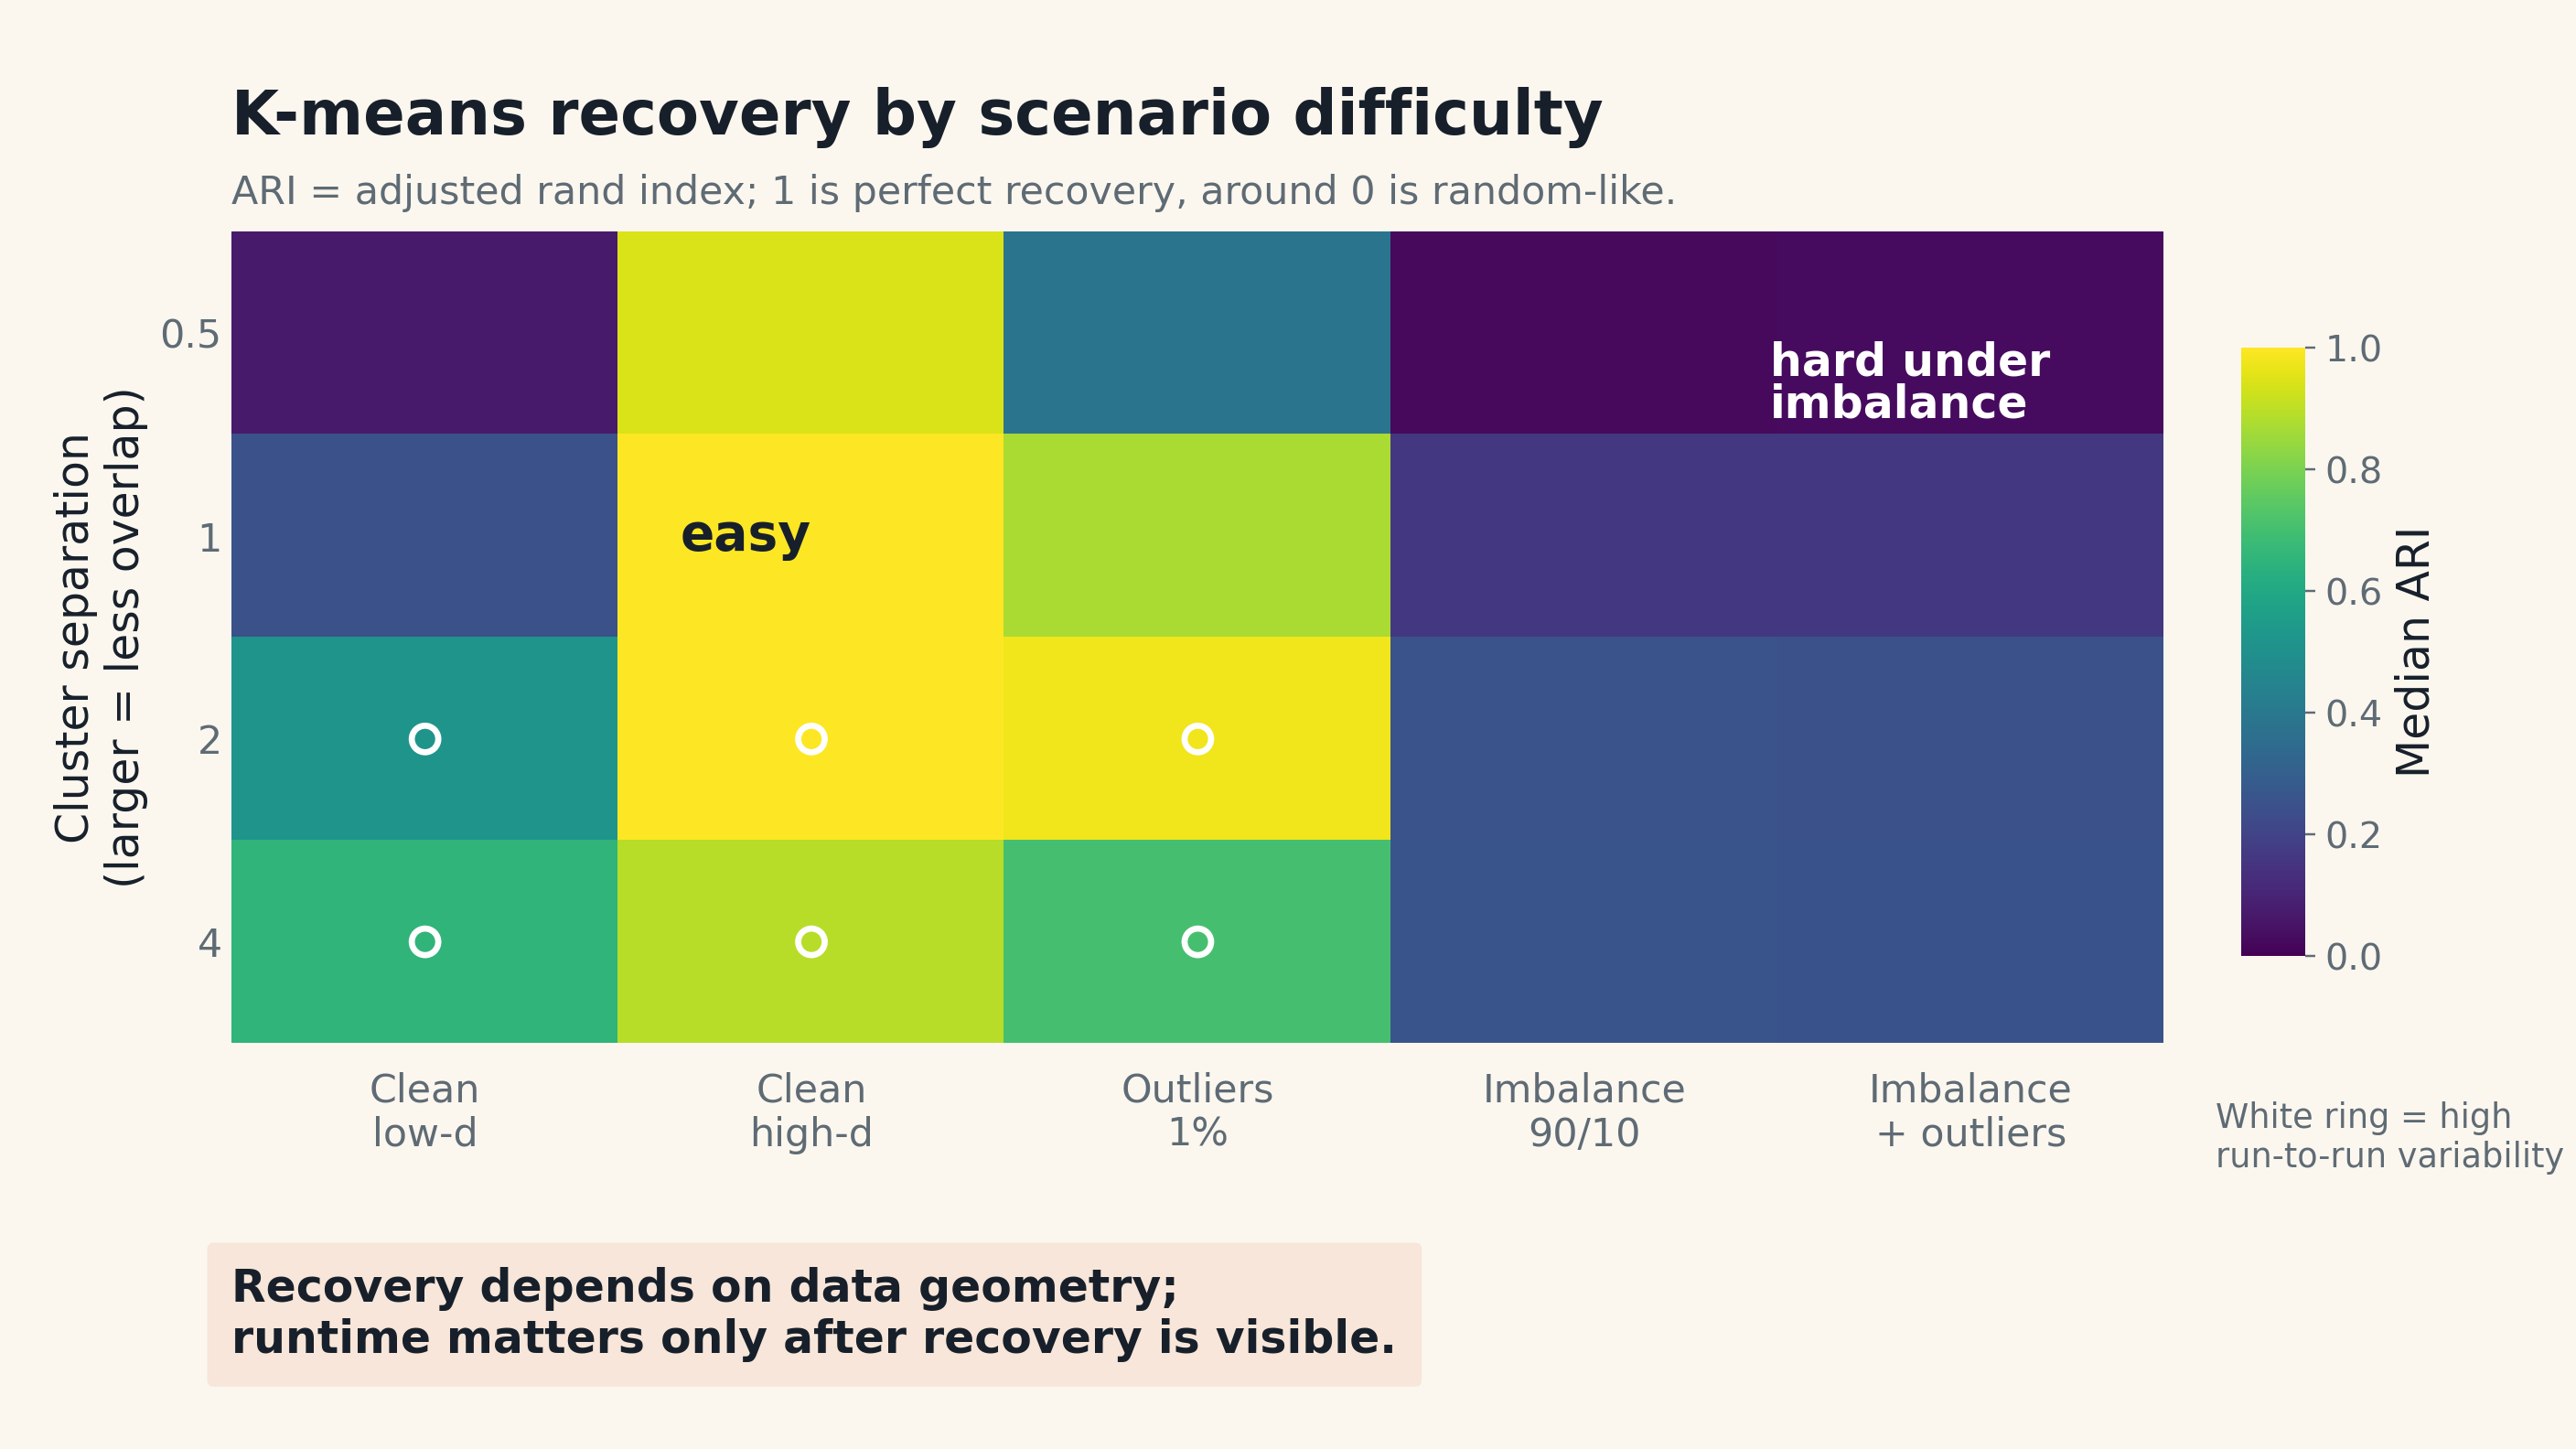
\includegraphics[width=0.98\linewidth]{../experiments/results/macbook_air_long/latest/figures/kmeans_recovery_scenario_facets.png}
    \end{figure}
    \captiontext{ARI = adjusted rand index. Runtime matters only after recovery is visible.}
  \end{block}

  \begin{alertblock}{Reference preservation}
    \begin{itemize}
      \item k-means optimized paths preserve inertia against the reference.
      \item permutation matrix paths preserve p-values against the loop.
      \item memory-risk skips are explicit rows, not hidden omissions.
    \end{itemize}
  \end{alertblock}
\end{column}

\separatorcolumn

\begin{column}{\colwidth}
  \begin{block}{Server CPU and A100: scale tier}
    \bigstat{numba}{540}{CPU k-means rows}
    \hfill
    \bigstat{jaxberry}{135}{A100 rows}
    \hfill
    \bigstat{cityumaroon}{5.8x}{A100 edge}

    \vspace{0.8em}
    \small
    Server results are interpreted as the next rung in the evidence ladder.
  \end{block}

  \begin{block}{k-means: shape-dependent acceleration}
    \begin{figure}
      \centering
      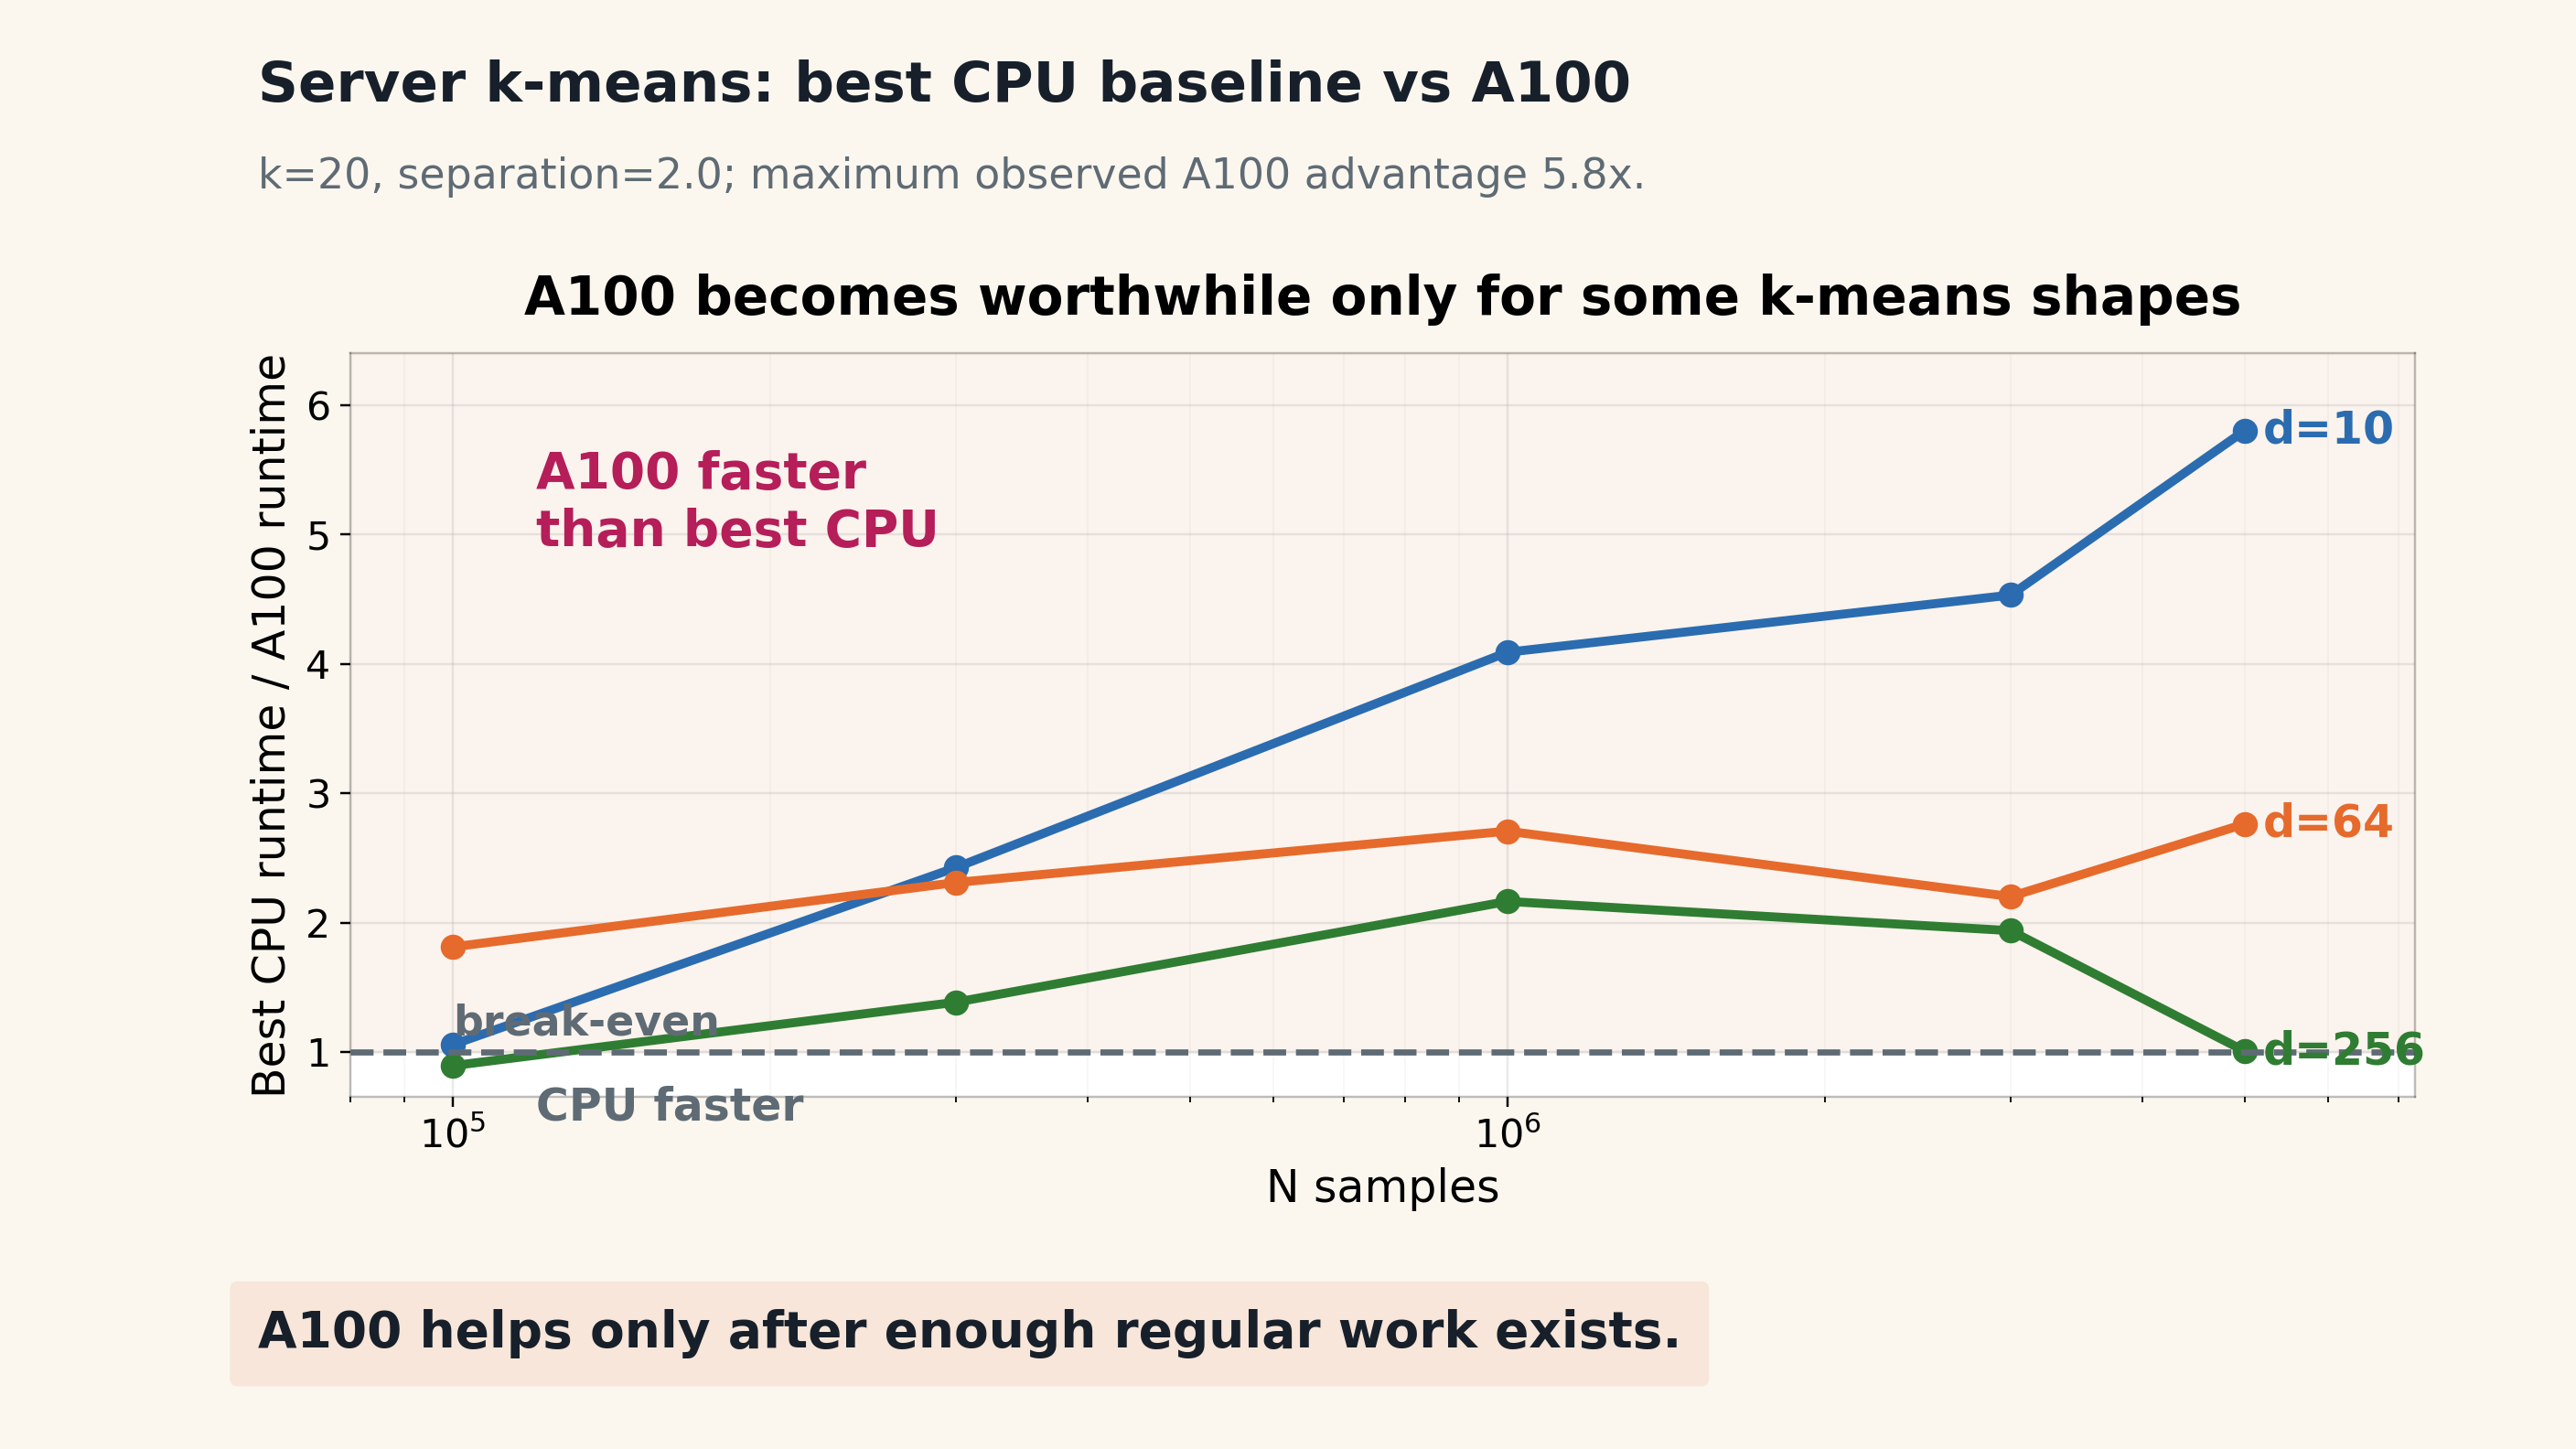
\includegraphics[width=0.98\linewidth]{../experiments/results/presentation_figures/server_kmeans_cpu_a100_summary.png}
    \end{figure}
    \captiontext{A100 helps only after enough regular array work exists.}
  \end{block}

  \begin{block}{Permutation: useful negative result}
    \begin{figure}
      \centering
      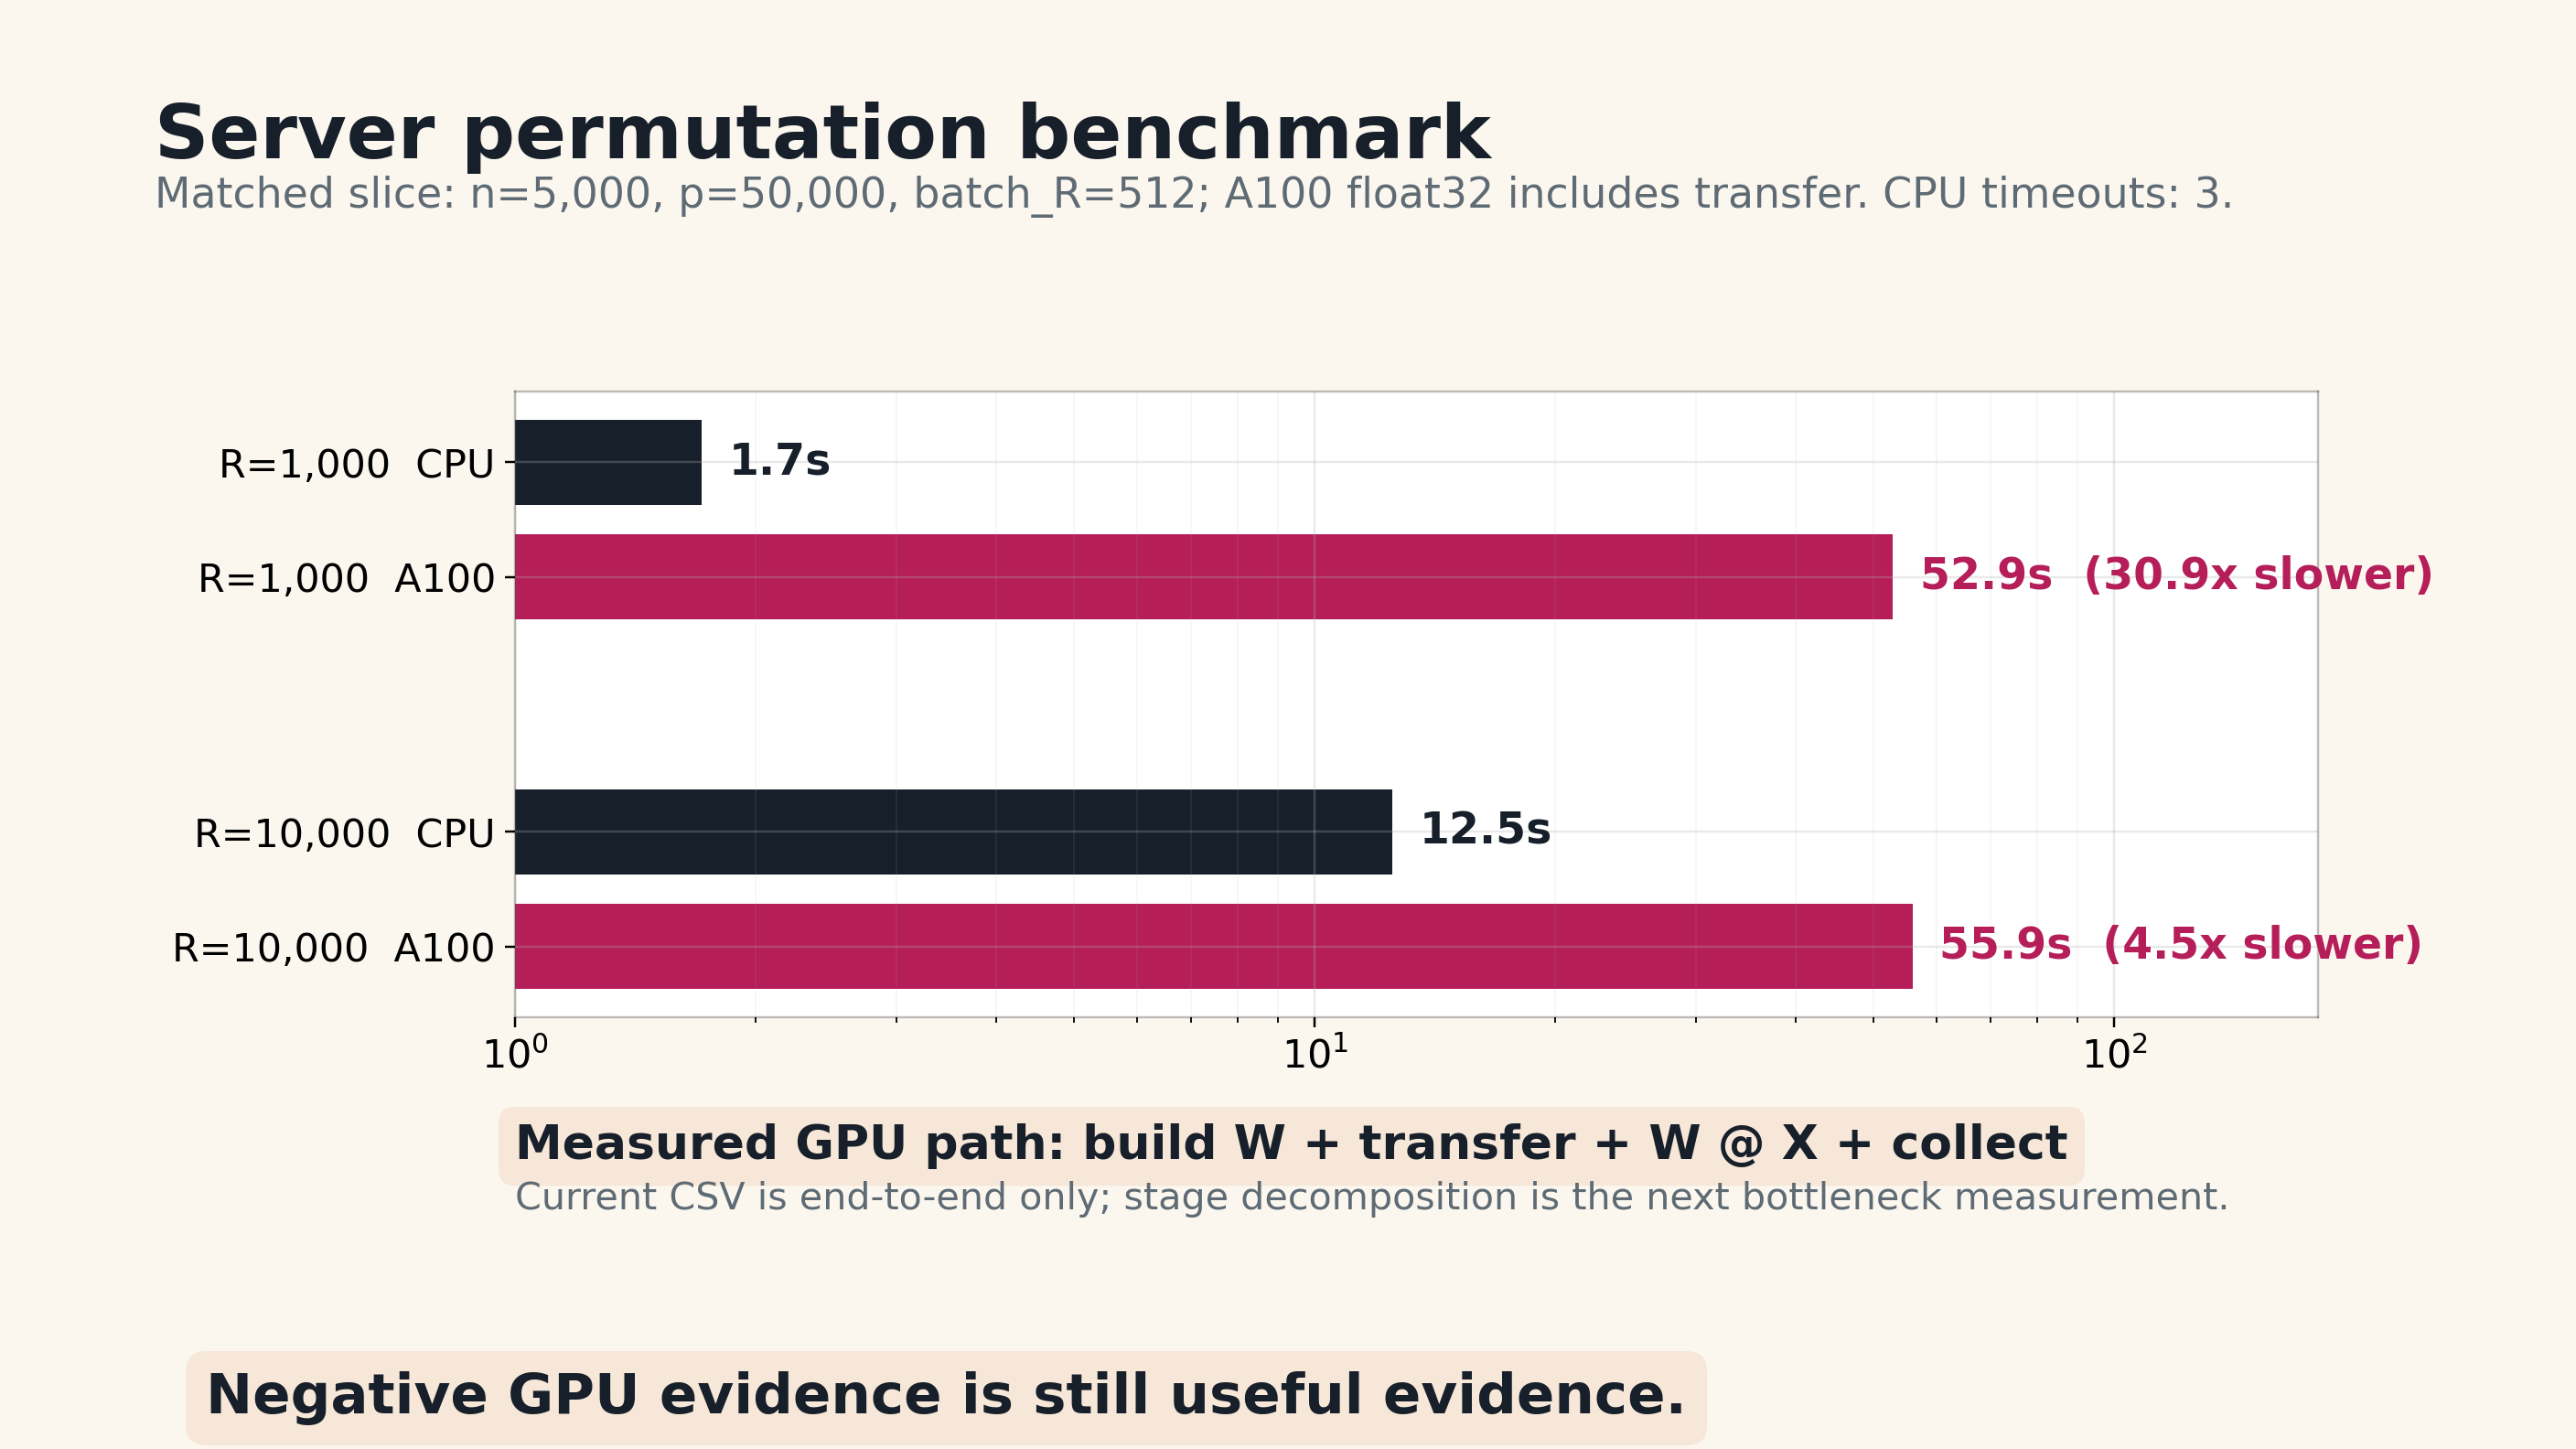
\includegraphics[width=0.98\linewidth]{../experiments/results/presentation_figures/server_permutation_cpu_a100_summary.png}
    \end{figure}
    \captiontext{Validated negative evidence: the matched A100 permutation path loses to CPU here.}
  \end{block}
\end{column}

\separatorcolumn

\begin{column}{\colwidth}
  \begin{block}{Parallelism must be tuned}
    \begin{figure}
      \centering
      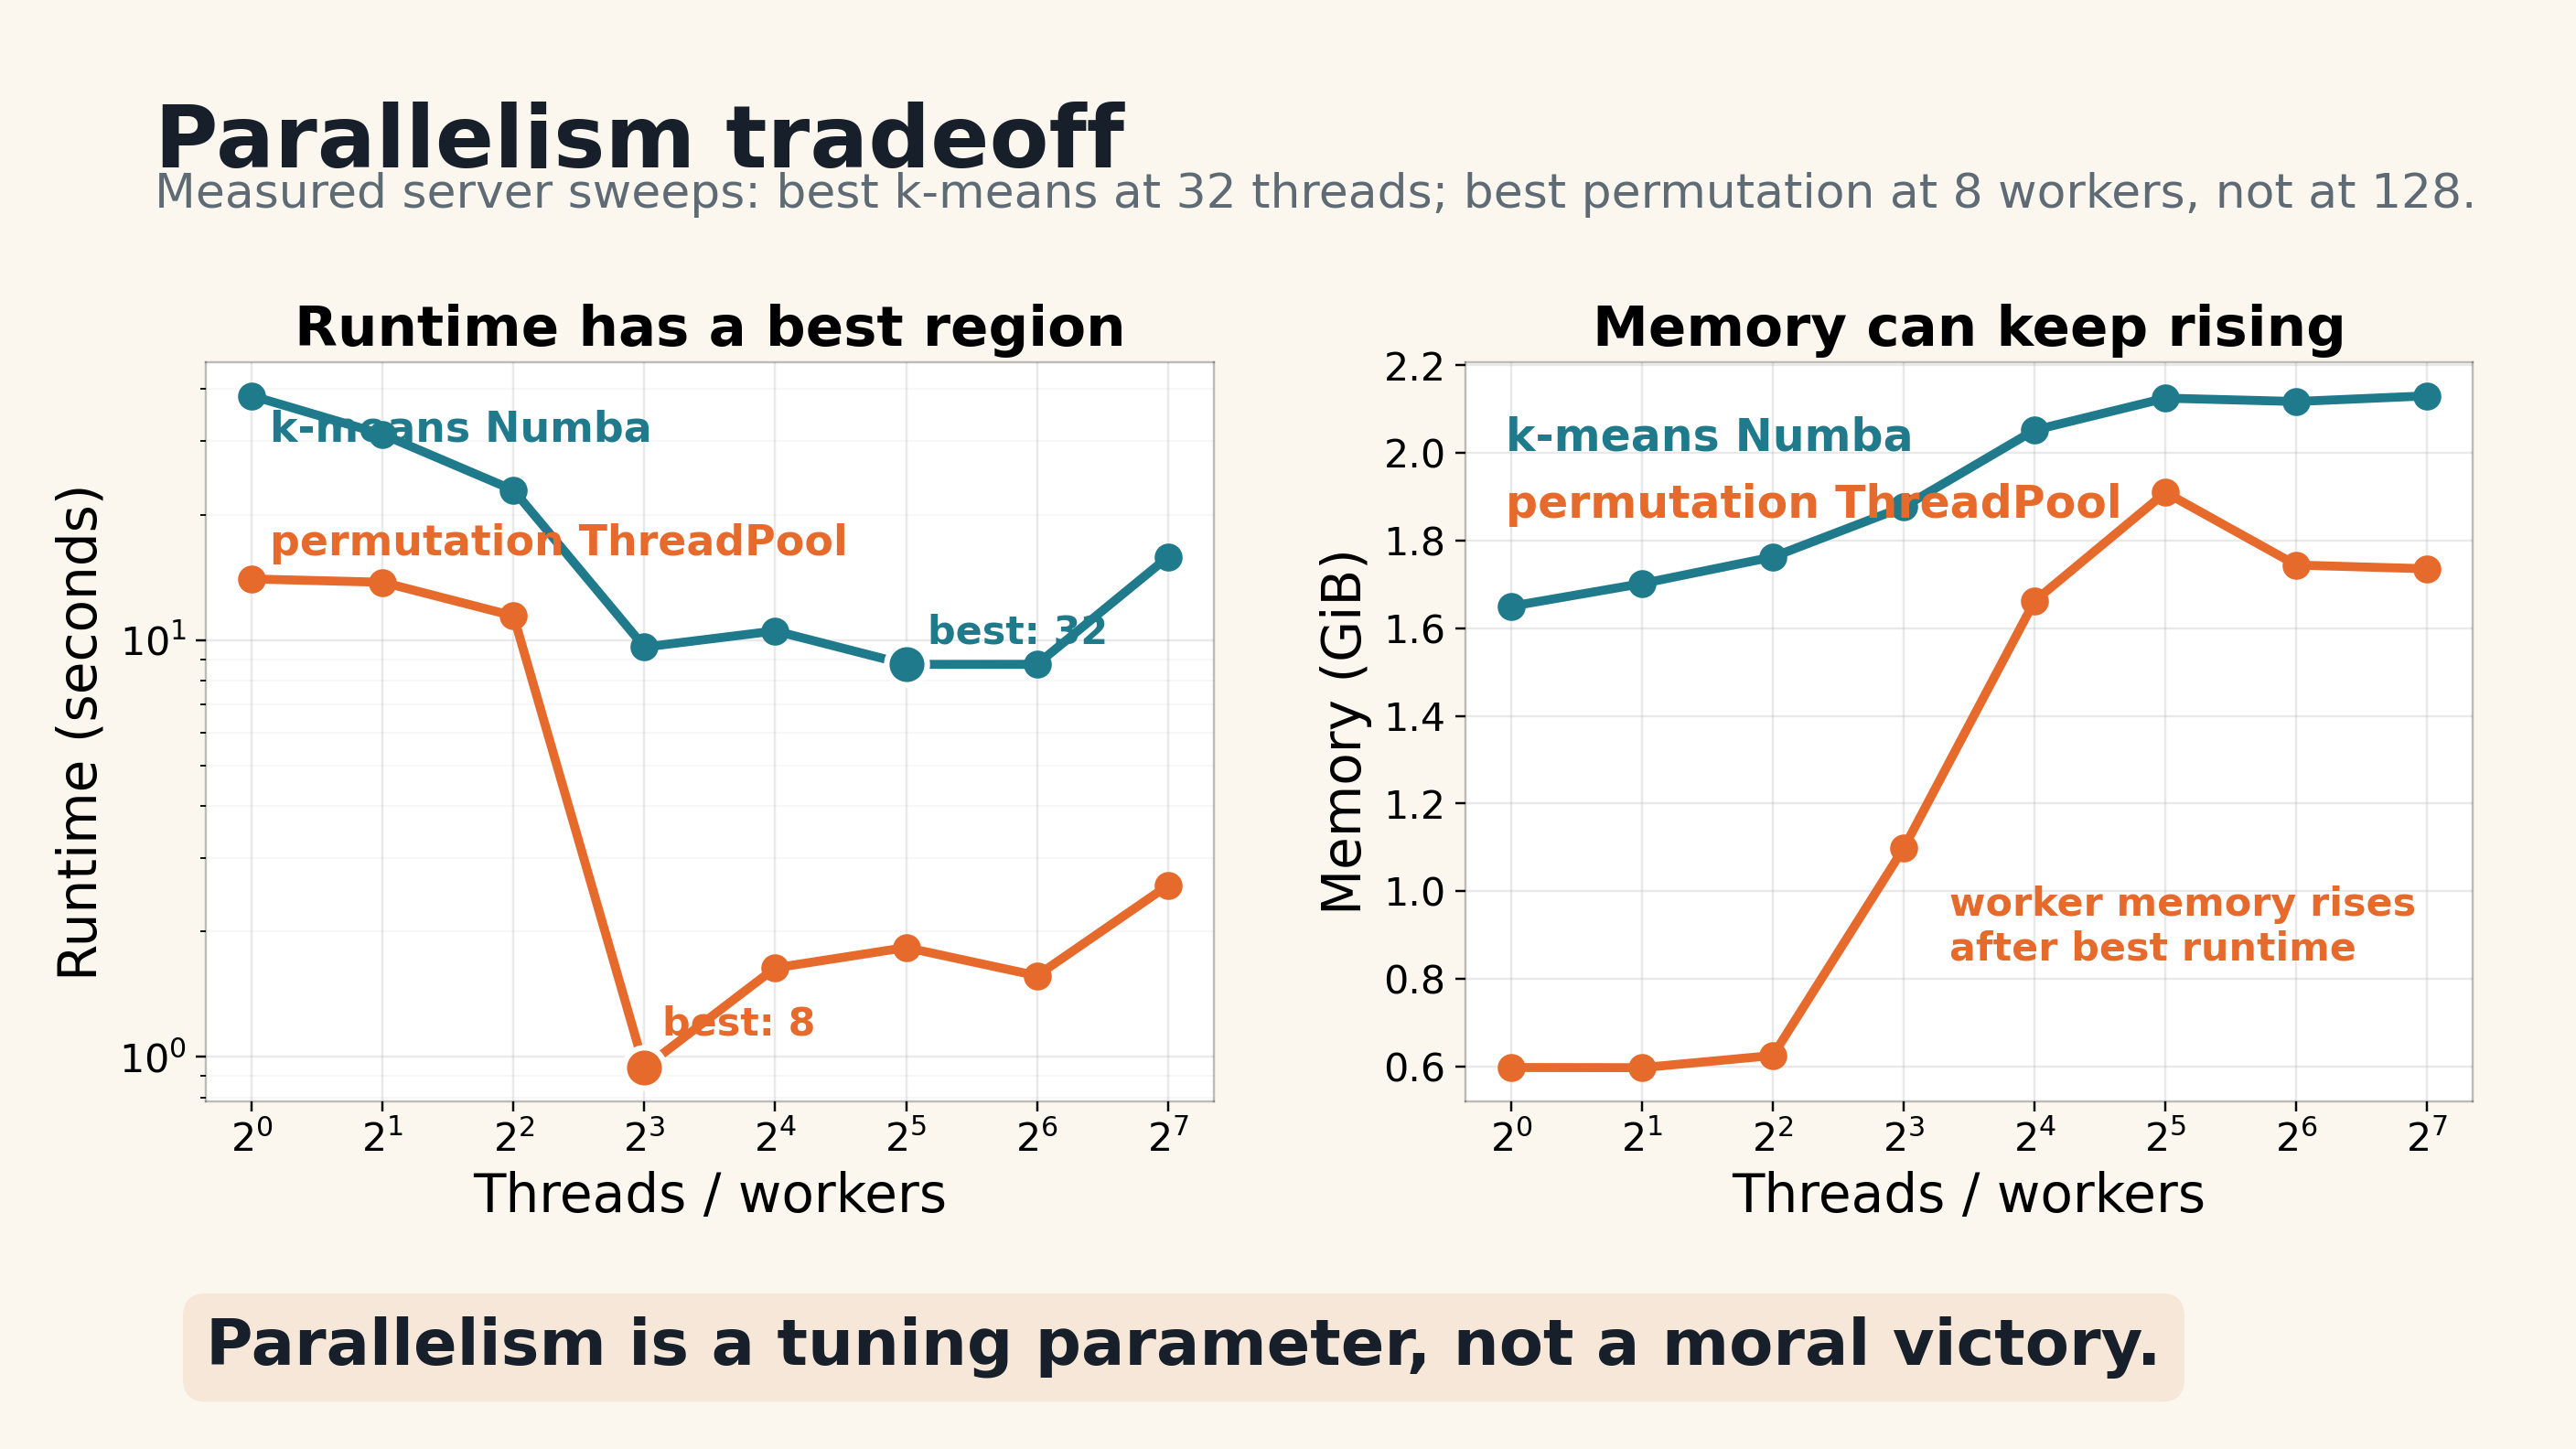
\includegraphics[width=0.98\linewidth]{../experiments/results/presentation_figures/server_parallelism_tradeoff.png}
    \end{figure}
    \captiontext{Best speed was not at maximum parallelism; memory can keep growing after runtime stops improving.}
  \end{block}

  \begin{block}{Memorable findings}
    \heading{Validate before optimizing}
    Faster code that changes the statistic is a different method.

    \vspace{0.65em}
    \heading{Shape beats logo}
    Numba, NumPy matmul, threads, and A100 each win on specific shapes.

    \vspace{0.65em}
    \heading{Negative GPU evidence is useful}
    It separates a valid formulation from a winning accelerator path.
  \end{block}

  \begin{alertblock}{Decision guide}
    \begin{itemize}
      \item Start with the clearest reference.
      \item Use Numba for hot scalar CPU loops.
      \item Use algebra before creating giant temporaries.
      \item Treat GPU as a formulation change.
    \end{itemize}

    \begin{center}
      {\Large\bfseries Clear enough to trust. Fast enough to scale.}

      \vspace{0.55em}
      {\Large\bfseries Evidence and slides}\\[-0.1em]
      {\large \texttt{github.com/lucajiang/}}\\[-0.05em]
      {\large \texttt{FastStatisticalModels4Python}}
    \end{center}
  \end{alertblock}
\end{column}

\separatorcolumn
\end{columns}

\vspace{0.35cm}
\begin{center}
\begin{minipage}{0.956\paperwidth}
  \begin{alertblock}{Talk spine}
    \begin{minipage}[t]{0.23\linewidth}
      \heading{1. Simulate truth}
      Build scenarios with known behavior.
    \end{minipage}
    \hfill
    \begin{minipage}[t]{0.23\linewidth}
      \heading{2. Preserve statistics}
      Check equivalence, calibration, and recovery.
    \end{minipage}
    \hfill
    \begin{minipage}[t]{0.23\linewidth}
      \heading{3. Scale evidence}
      Move laptop to server CPU to A100.
    \end{minipage}
    \hfill
    \begin{minipage}[t]{0.23\linewidth}
      \heading{4. Pick the smallest tool}
      Pick the tool that removes the proven bottleneck.
    \end{minipage}
  \end{alertblock}
\end{minipage}
\end{center}

\vspace{0.08cm}
\begin{center}
{\footnotesize\color{muted}
Evidence pack: \texttt{macbook\_air\_long/latest} \quad
\texttt{linux\_server\_cpu/long\_safe\_20260503\_190133} \quad
\texttt{linux\_server\_a100/long\_safe\_20260503\_190133}}
\end{center}
\end{frame}
\end{document}
